%%%%%%%%%%%%%%%%%%%%%%%%%%%%%%%%%%%%%%%%%
% The Legrand Orange Book
% LaTeX Template
% Version 2.1.1 (14/2/16)
%
% This template has been downloaded from:
% http://www.LaTeXTemplates.com
%
% Original author:
% Mathias Legrand (legrand.mathias@gmail.com) with modifications by:
% Vel (vel@latextemplates.com)
%
% License:
% CC BY-NC-SA 3.0 (http://creativecommons.org/licenses/by-nc-sa/3.0/)
%
% Compiling this template:
% This template uses biber for its bibliography and makeindex for its index.
% When you first open the template, compile it from the command line with the 
% commands below to make sure your LaTeX distribution is configured correctly:
%
% 1) pdflatex main
% 2) makeindex main.idx -s StyleInd.ist
% 3) biber main
% 4) pdflatex main x 2
%
% After this, when you wish to update the bibliography/index use the appropriate
% command above and make sure to compile with pdflatex several times 
% afterwards to propagate your changes to the document.
%
% This template also uses a number of packages which may need to be
% updated to the newest versions for the template to compile. It is strongly
% recommended you update your LaTeX distribution if you have any
% compilation errors.
%
% Important note:
% Chapter heading images should have a 2:1 width:height ratio,
% e.g. 920px width and 460px height.
%
%%%%%%%%%%%%%%%%%%%%%%%%%%%%%%%%%%%%%%%%%

%----------------------------------------------------------------------------------------
%	PACKAGES AND OTHER DOCUMENT CONFIGURATIONS
%----------------------------------------------------------------------------------------

\documentclass[11pt,fleqn]{book} % Default font size and left-justified equations
\usepackage{wrapfig}
\usepackage{listings}
%----------------------------------------------------------------------------------------

%%%%%%%%%%%%%%%%%%%%%%%%%%%%%%%%%%%%%%%%%
% The Legrand Orange Book
% Structural Definitions File
% Version 2.0 (9/2/15)
%
% Original author:
% Mathias Legrand (legrand.mathias@gmail.com) with modifications by:
% Vel (vel@latextemplates.com)
% 
% This file has been downloaded from:
% http://www.LaTeXTemplates.com
%
% License:
% CC BY-NC-SA 3.0 (http://creativecommons.org/licenses/by-nc-sa/3.0/)
%
%%%%%%%%%%%%%%%%%%%%%%%%%%%%%%%%%%%%%%%%%

%----------------------------------------------------------------------------------------
%	VARIOUS REQUIRED PACKAGES AND CONFIGURATIONS
%----------------------------------------------------------------------------------------

\usepackage[top=3cm,bottom=3cm,left=3cm,right=3cm,headsep=10pt,a4paper]{geometry} % Page margins

\usepackage{graphicx} % Required for including pictures
\graphicspath{{Pictures/}} % Specifies the directory where pictures are stored

\usepackage{lipsum} % Inserts dummy text

\usepackage{tikz} % Required for drawing custom shapes

\usepackage[english]{babel} % English language/hyphenation

\usepackage{enumitem} % Customize lists
\setlist{nolistsep} % Reduce spacing between bullet points and numbered lists

\usepackage{booktabs} % Required for nicer horizontal rules in tables

\usepackage{xcolor} % Required for specifying colors by name
%\definecolor{ocre}{RGB}{243,102,25} % Define the orange color used for highlighting throughout the book (Original)
\definecolor{ocre}{RGB}{0,135,180} % This is actually a kind of blue

%----------------------------------------------------------------------------------------
%	FONTS
%----------------------------------------------------------------------------------------

\usepackage{avant} % Use the Avantgarde font for headings
%\usepackage{times} % Use the Times font for headings
\usepackage{mathptmx} % Use the Adobe Times Roman as the default text font together with math symbols from the Sym­bol, Chancery and Com­puter Modern fonts

\usepackage{microtype} % Slightly tweak font spacing for aesthetics
\usepackage[utf8]{inputenc} % Required for including letters with accents
\usepackage[T1]{fontenc} % Use 8-bit encoding that has 256 glyphs

%----------------------------------------------------------------------------------------
%	BIBLIOGRAPHY AND INDEX
%----------------------------------------------------------------------------------------

\usepackage[style=alphabetic,citestyle=numeric,sorting=nyt,sortcites=true,autopunct=true,babel=hyphen,hyperref=true,abbreviate=false,backref=true,backend=biber]{biblatex}
\addbibresource{bibliography.bib} % BibTeX bibliography file
\defbibheading{bibempty}{}

\usepackage{calc} % For simpler calculation - used for spacing the index letter headings correctly
\usepackage{makeidx} % Required to make an index
\makeindex % Tells LaTeX to create the files required for indexing

%----------------------------------------------------------------------------------------
%	MAIN TABLE OF CONTENTS
%----------------------------------------------------------------------------------------

\usepackage{titletoc} % Required for manipulating the table of contents

\contentsmargin{0cm} % Removes the default margin

% Part text styling
\titlecontents{part}[0cm]
{\addvspace{20pt}\centering\large\bfseries}
{}
{}
{}

% Chapter text styling
\titlecontents{chapter}[1.25cm] % Indentation
{\addvspace{12pt}\large\sffamily\bfseries} % Spacing and font options for chapters
{\color{ocre!60}\contentslabel[\Large\thecontentslabel]{1.25cm}\color{ocre}} % Chapter number
{\color{ocre}}  
{\color{ocre!60}\normalsize\;\titlerule*[.5pc]{.}\;\thecontentspage} % Page number

% Section text styling
\titlecontents{section}[1.25cm] % Indentation
{\addvspace{3pt}\sffamily\bfseries} % Spacing and font options for sections
{\contentslabel[\thecontentslabel]{1.25cm}} % Section number
{}
{\hfill\color{black}\thecontentspage} % Page number
[]

% Subsection text styling
\titlecontents{subsection}[1.25cm] % Indentation
{\addvspace{1pt}\sffamily\small} % Spacing and font options for subsections
{\contentslabel[\thecontentslabel]{1.25cm}} % Subsection number
{}
{\ \titlerule*[.5pc]{.}\;\thecontentspage} % Page number
[]

% List of figures
\titlecontents{figure}[0em]
{\addvspace{-5pt}\sffamily}
{\thecontentslabel\hspace*{1em}}
{}
{\ \titlerule*[.5pc]{.}\;\thecontentspage}
[]

% List of tables
\titlecontents{table}[0em]
{\addvspace{-5pt}\sffamily}
{\thecontentslabel\hspace*{1em}}
{}
{\ \titlerule*[.5pc]{.}\;\thecontentspage}
[]

%----------------------------------------------------------------------------------------
%	MINI TABLE OF CONTENTS IN PART HEADS
%----------------------------------------------------------------------------------------

% Chapter text styling
\titlecontents{lchapter}[0em] % Indenting
{\addvspace{15pt}\large\sffamily\bfseries} % Spacing and font options for chapters
{\color{ocre}\contentslabel[\Large\thecontentslabel]{1.25cm}\color{ocre}} % Chapter number
{}  
{\color{ocre}\normalsize\sffamily\bfseries\;\titlerule*[.5pc]{.}\;\thecontentspage} % Page number

% Section text styling
\titlecontents{lsection}[0em] % Indenting
{\sffamily\small} % Spacing and font options for sections
{\contentslabel[\thecontentslabel]{1.25cm}} % Section number
{}
{}

% Subsection text styling
\titlecontents{lsubsection}[.5em] % Indentation
{\normalfont\footnotesize\sffamily} % Font settings
{}
{}
{}

%----------------------------------------------------------------------------------------
%	PAGE HEADERS
%----------------------------------------------------------------------------------------

\usepackage{fancyhdr} % Required for header and footer configuration

\pagestyle{fancy}
\renewcommand{\chaptermark}[1]{\markboth{\sffamily\normalsize\bfseries\chaptername\ \thechapter.\ #1}{}} % Chapter text font settings
\renewcommand{\sectionmark}[1]{\markright{\sffamily\normalsize\thesection\hspace{5pt}#1}{}} % Section text font settings
\fancyhf{} \fancyhead[LE,RO]{\sffamily\normalsize\thepage} % Font setting for the page number in the header
\fancyhead[LO]{\rightmark} % Print the nearest section name on the left side of odd pages
\fancyhead[RE]{\leftmark} % Print the current chapter name on the right side of even pages
\renewcommand{\headrulewidth}{0.5pt} % Width of the rule under the header
\addtolength{\headheight}{2.5pt} % Increase the spacing around the header slightly
\renewcommand{\footrulewidth}{0pt} % Removes the rule in the footer
\fancypagestyle{plain}{\fancyhead{}\renewcommand{\headrulewidth}{0pt}} % Style for when a plain pagestyle is specified

% Removes the header from odd empty pages at the end of chapters
\makeatletter
\renewcommand{\cleardoublepage}{
\clearpage\ifodd\c@page\else
\hbox{}
\vspace*{\fill}
\thispagestyle{empty}
\newpage
\fi}

%----------------------------------------------------------------------------------------
%	THEOREM STYLES
%----------------------------------------------------------------------------------------

\usepackage{amsmath,amsfonts,amssymb,amsthm} % For math equations, theorems, symbols, etc

\newcommand{\intoo}[2]{\mathopen{]}#1\,;#2\mathclose{[}}
\newcommand{\ud}{\mathop{\mathrm{{}d}}\mathopen{}}
\newcommand{\intff}[2]{\mathopen{[}#1\,;#2\mathclose{]}}
\newtheorem{notation}{Notation}[chapter]

% Boxed/framed environments
\newtheoremstyle{ocrenumbox}% % Theorem style name
{0pt}% Space above
{0pt}% Space below
{\normalfont}% % Body font
{}% Indent amount
{\small\bf\sffamily\color{ocre}}% % Theorem head font
{\;}% Punctuation after theorem head
{0.25em}% Space after theorem head
{\small\sffamily\color{ocre}\thmname{#1}\nobreakspace\thmnumber{\@ifnotempty{#1}{}\@upn{#2}}% Theorem text (e.g. Theorem 2.1)
\thmnote{\nobreakspace\the\thm@notefont\sffamily\bfseries\color{black}---\nobreakspace#3.}} % Optional theorem note
\renewcommand{\qedsymbol}{$\blacksquare$}% Optional qed square

\newtheoremstyle{blacknumex}% Theorem style name
{5pt}% Space above
{5pt}% Space below
{\normalfont}% Body font
{} % Indent amount
{\small\bf\sffamily}% Theorem head font
{\;}% Punctuation after theorem head
{0.25em}% Space after theorem head
{\small\sffamily{\tiny\ensuremath{\blacksquare}}\nobreakspace\thmname{#1}\nobreakspace\thmnumber{\@ifnotempty{#1}{}\@upn{#2}}% Theorem text (e.g. Theorem 2.1)
\thmnote{\nobreakspace\the\thm@notefont\sffamily\bfseries---\nobreakspace#3.}}% Optional theorem note

\newtheoremstyle{blacknumbox} % Theorem style name
{0pt}% Space above
{0pt}% Space below
{\normalfont}% Body font
{}% Indent amount
{\small\bf\sffamily}% Theorem head font
{\;}% Punctuation after theorem head
{0.25em}% Space after theorem head
{\small\sffamily\thmname{#1}\nobreakspace\thmnumber{\@ifnotempty{#1}{}\@upn{#2}}% Theorem text (e.g. Theorem 2.1)
\thmnote{\nobreakspace\the\thm@notefont\sffamily\bfseries---\nobreakspace#3.}}% Optional theorem note

% Non-boxed/non-framed environments
\newtheoremstyle{ocrenum}% % Theorem style name
{5pt}% Space above
{5pt}% Space below
{\normalfont}% % Body font
{}% Indent amount
{\small\bf\sffamily\color{ocre}}% % Theorem head font
{\;}% Punctuation after theorem head
{0.25em}% Space after theorem head
{\small\sffamily\color{ocre}\thmname{#1}\nobreakspace\thmnumber{\@ifnotempty{#1}{}\@upn{#2}}% Theorem text (e.g. Theorem 2.1)
\thmnote{\nobreakspace\the\thm@notefont\sffamily\bfseries\color{black}---\nobreakspace#3.}} % Optional theorem note
\renewcommand{\qedsymbol}{$\blacksquare$}% Optional qed square
\makeatother

% Defines the theorem text style for each type of theorem to one of the three styles above
\newcounter{dummy} 
\numberwithin{dummy}{section}
\theoremstyle{ocrenumbox}
\newtheorem{theoremeT}[dummy]{Theorem}
\newtheorem{problem}{Problem}[chapter]
\newtheorem{exerciseT}{Exercise}[chapter]
\theoremstyle{blacknumex}
\newtheorem{exampleT}{Example}[chapter]
\theoremstyle{blacknumbox}
\newtheorem{vocabulary}{Vocabulary}[chapter]
\newtheorem{definitionT}{Definition}[section]
\newtheorem{corollaryT}[dummy]{Corollary}
\theoremstyle{ocrenum}
\newtheorem{proposition}[dummy]{Proposition}

%----------------------------------------------------------------------------------------
%	DEFINITION OF COLORED BOXES
%----------------------------------------------------------------------------------------

\RequirePackage[framemethod=default]{mdframed} % Required for creating the theorem, definition, exercise and corollary boxes

% Theorem box
\newmdenv[skipabove=7pt,
skipbelow=7pt,
backgroundcolor=black!5,
linecolor=ocre,
innerleftmargin=5pt,
innerrightmargin=5pt,
innertopmargin=5pt,
leftmargin=0cm,
rightmargin=0cm,
innerbottommargin=5pt]{tBox}

% Exercise box	  
\newmdenv[skipabove=7pt,
skipbelow=7pt,
rightline=false,
leftline=true,
topline=false,
bottomline=false,
backgroundcolor=ocre!10,
linecolor=ocre,
innerleftmargin=5pt,
innerrightmargin=5pt,
innertopmargin=5pt,
innerbottommargin=5pt,
leftmargin=0cm,
rightmargin=0cm,
linewidth=4pt]{eBox}	

% Definition box
\newmdenv[skipabove=7pt,
skipbelow=7pt,
rightline=false,
leftline=true,
topline=false,
bottomline=false,
linecolor=ocre,
innerleftmargin=5pt,
innerrightmargin=5pt,
innertopmargin=0pt,
leftmargin=0cm,
rightmargin=0cm,
linewidth=4pt,
innerbottommargin=0pt]{dBox}	

% Corollary box
\newmdenv[skipabove=7pt,
skipbelow=7pt,
rightline=false,
leftline=true,
topline=false,
bottomline=false,
linecolor=gray,
backgroundcolor=black!5,
innerleftmargin=5pt,
innerrightmargin=5pt,
innertopmargin=5pt,
leftmargin=0cm,
rightmargin=0cm,
linewidth=4pt,
innerbottommargin=5pt]{cBox}

% Creates an environment for each type of theorem and assigns it a theorem text style from the "Theorem Styles" section above and a colored box from above
\newenvironment{theorem}{\begin{tBox}\begin{theoremeT}}{\end{theoremeT}\end{tBox}}
\newenvironment{exercise}{\begin{eBox}\begin{exerciseT}}{\hfill{\color{ocre}\tiny\ensuremath{\blacksquare}}\end{exerciseT}\end{eBox}}				  
\newenvironment{definition}{\begin{dBox}\begin{definitionT}}{\end{definitionT}\end{dBox}}	
\newenvironment{example}{\begin{exampleT}}{\hfill{\tiny\ensuremath{\blacksquare}}\end{exampleT}}		
\newenvironment{corollary}{\begin{cBox}\begin{corollaryT}}{\end{corollaryT}\end{cBox}}	

%----------------------------------------------------------------------------------------
%	REMARK ENVIRONMENT
%----------------------------------------------------------------------------------------

\newenvironment{remark}{\par\vspace{10pt}\small % Vertical white space above the remark and smaller font size
\begin{list}{}{
\leftmargin=35pt % Indentation on the left
\rightmargin=25pt}\item\ignorespaces % Indentation on the right
\makebox[-2.5pt]{\begin{tikzpicture}[overlay]
\node[draw=ocre!60,line width=1pt,circle,fill=ocre!25,font=\sffamily\bfseries,inner sep=2pt,outer sep=0pt] at (-15pt,0pt){\textcolor{ocre}{R}};\end{tikzpicture}} % Orange R in a circle
\advance\baselineskip -1pt}{\end{list}\vskip5pt} % Tighter line spacing and white space after remark

%----------------------------------------------------------------------------------------
%	SECTION NUMBERING IN THE MARGIN
%----------------------------------------------------------------------------------------

\makeatletter
\renewcommand{\@seccntformat}[1]{\llap{\textcolor{ocre}{\csname the#1\endcsname}\hspace{1em}}}                    
\renewcommand{\section}{\@startsection{section}{1}{\z@}
{-4ex \@plus -1ex \@minus -.4ex}
{1ex \@plus.2ex }
{\normalfont\large\sffamily\bfseries}}
\renewcommand{\subsection}{\@startsection {subsection}{2}{\z@}
{-3ex \@plus -0.1ex \@minus -.4ex}
{0.5ex \@plus.2ex }
{\normalfont\sffamily\bfseries}}
\renewcommand{\subsubsection}{\@startsection {subsubsection}{3}{\z@}
{-2ex \@plus -0.1ex \@minus -.2ex}
{.2ex \@plus.2ex }
{\normalfont\small\sffamily\bfseries}}                        
\renewcommand\paragraph{\@startsection{paragraph}{4}{\z@}
{-2ex \@plus-.2ex \@minus .2ex}
{.1ex}
{\normalfont\small\sffamily\bfseries}}

%----------------------------------------------------------------------------------------
%	PART HEADINGS
%----------------------------------------------------------------------------------------

% numbered part in the table of contents
\newcommand{\@mypartnumtocformat}[2]{%
\setlength\fboxsep{0pt}%
\noindent\colorbox{ocre!20}{\strut\parbox[c][.7cm]{\ecart}{\color{ocre!70}\Large\sffamily\bfseries\centering#1}}\hskip\esp\colorbox{ocre!40}{\strut\parbox[c][.7cm]{\linewidth-\ecart-\esp}{\Large\sffamily\centering#2}}}%
%%%%%%%%%%%%%%%%%%%%%%%%%%%%%%%%%%
% unnumbered part in the table of contents
\newcommand{\@myparttocformat}[1]{%
\setlength\fboxsep{0pt}%
\noindent\colorbox{ocre!40}{\strut\parbox[c][.7cm]{\linewidth}{\Large\sffamily\centering#1}}}%
%%%%%%%%%%%%%%%%%%%%%%%%%%%%%%%%%%
\newlength\esp
\setlength\esp{4pt}
\newlength\ecart
\setlength\ecart{1.2cm-\esp}
\newcommand{\thepartimage}{}%
\newcommand{\partimage}[1]{\renewcommand{\thepartimage}{#1}}%
\def\@part[#1]#2{%
\ifnum \c@secnumdepth >-2\relax%
\refstepcounter{part}%
\addcontentsline{toc}{part}{\texorpdfstring{\protect\@mypartnumtocformat{\thepart}{#1}}{\partname~\thepart\ ---\ #1}}
\else%
\addcontentsline{toc}{part}{\texorpdfstring{\protect\@myparttocformat{#1}}{#1}}%
\fi%
\startcontents%
\markboth{}{}%
{\thispagestyle{empty}%
\begin{tikzpicture}[remember picture,overlay]%
\node at (current page.north west){\begin{tikzpicture}[remember picture,overlay]%	
\fill[ocre!20](0cm,0cm) rectangle (\paperwidth,-\paperheight);
\node[anchor=north] at (4cm,-3.25cm){\color{ocre!40}\fontsize{220}{100}\sffamily\bfseries\@Roman\c@part}; 
\node[anchor=south east] at (\paperwidth-1cm,-\paperheight+1cm){\parbox[t][][t]{8.5cm}{
\printcontents{l}{0}{\setcounter{tocdepth}{1}}%
}};
\node[anchor=north east] at (\paperwidth-1.5cm,-3.25cm){\parbox[t][][t]{15cm}{\strut\raggedleft\color{white}\fontsize{30}{30}\sffamily\bfseries#2}};
\end{tikzpicture}};
\end{tikzpicture}}%
\@endpart}
\def\@spart#1{%
\startcontents%
\phantomsection
{\thispagestyle{empty}%
\begin{tikzpicture}[remember picture,overlay]%
\node at (current page.north west){\begin{tikzpicture}[remember picture,overlay]%	
\fill[ocre!20](0cm,0cm) rectangle (\paperwidth,-\paperheight);
\node[anchor=north east] at (\paperwidth-1.5cm,-3.25cm){\parbox[t][][t]{15cm}{\strut\raggedleft\color{white}\fontsize{30}{30}\sffamily\bfseries#1}};
\end{tikzpicture}};
\end{tikzpicture}}
\addcontentsline{toc}{part}{\texorpdfstring{%
\setlength\fboxsep{0pt}%
\noindent\protect\colorbox{ocre!40}{\strut\protect\parbox[c][.7cm]{\linewidth}{\Large\sffamily\protect\centering #1\quad\mbox{}}}}{#1}}%
\@endpart}
\def\@endpart{\vfil\newpage
\if@twoside
\if@openright
\null
\thispagestyle{empty}%
\newpage
\fi
\fi
\if@tempswa
\twocolumn
\fi}

%----------------------------------------------------------------------------------------
%	CHAPTER HEADINGS
%----------------------------------------------------------------------------------------

% A switch to conditionally include a picture, implemented by  Christian Hupfer
\newif\ifusechapterimage
\usechapterimagetrue
\newcommand{\thechapterimage}{}%
\newcommand{\chapterimage}[1]{\ifusechapterimage\renewcommand{\thechapterimage}{#1}\fi}%
\def\@makechapterhead#1{%
{\parindent \z@ \raggedright \normalfont
\ifnum \c@secnumdepth >\m@ne
\if@mainmatter
\begin{tikzpicture}[remember picture,overlay]
\node at (current page.north west)
{\begin{tikzpicture}[remember picture,overlay]
\node[anchor=north west,inner sep=0pt] at (0,0) {\ifusechapterimage\includegraphics[width=\paperwidth]{\thechapterimage}\fi};
\draw[anchor=west] (\Gm@lmargin,-9cm) node [line width=2pt,rounded corners=15pt,draw=ocre,fill=white,fill opacity=0.5,inner sep=15pt]{\strut\makebox[22cm]{}};
\draw[anchor=west] (\Gm@lmargin+.3cm,-9cm) node {\huge\sffamily\bfseries\color{black}\thechapter. #1\strut};
\end{tikzpicture}};
\end{tikzpicture}
\else
\begin{tikzpicture}[remember picture,overlay]
\node at (current page.north west)
{\begin{tikzpicture}[remember picture,overlay]
\node[anchor=north west,inner sep=0pt] at (0,0) {\ifusechapterimage\includegraphics[width=\paperwidth]{\thechapterimage}\fi};
\draw[anchor=west] (\Gm@lmargin,-9cm) node [line width=2pt,rounded corners=15pt,draw=ocre,fill=white,fill opacity=0.5,inner sep=15pt]{\strut\makebox[22cm]{}};
\draw[anchor=west] (\Gm@lmargin+.3cm,-9cm) node {\huge\sffamily\bfseries\color{black}#1\strut};
\end{tikzpicture}};
\end{tikzpicture}
\fi\fi\par\vspace*{270\p@}}}

%-------------------------------------------

\def\@makeschapterhead#1{%
\begin{tikzpicture}[remember picture,overlay]
\node at (current page.north west)
{\begin{tikzpicture}[remember picture,overlay]
\node[anchor=north west,inner sep=0pt] at (0,0) {\ifusechapterimage\includegraphics[width=\paperwidth]{\thechapterimage}\fi};
\draw[anchor=west] (\Gm@lmargin,-9cm) node [line width=2pt,rounded corners=15pt,draw=ocre,fill=white,fill opacity=0.5,inner sep=15pt]{\strut\makebox[22cm]{}};
\draw[anchor=west] (\Gm@lmargin+.3cm,-9cm) node {\huge\sffamily\bfseries\color{black}#1\strut};
\end{tikzpicture}};
\end{tikzpicture}
\par\vspace*{270\p@}}
\makeatother

%----------------------------------------------------------------------------------------
%	HYPERLINKS IN THE DOCUMENTS
%----------------------------------------------------------------------------------------

\usepackage{hyperref}
\hypersetup{hidelinks,backref=true,pagebackref=true,hyperindex=true,colorlinks=false,breaklinks=true,urlcolor= ocre,bookmarks=true,bookmarksopen=false,pdftitle={Title},pdfauthor={Author}}
\usepackage{bookmark}
\bookmarksetup{
open,
numbered,
addtohook={%
\ifnum\bookmarkget{level}=0 % chapter
\bookmarksetup{bold}%
\fi
\ifnum\bookmarkget{level}=-1 % part
\bookmarksetup{color=ocre,bold}%
\fi
}
}
 % Insert the commands.tex file which contains the majority of the structure behind the template

\begin{document}

%----------------------------------------------------------------------------------------
%	TITLE PAGE
%----------------------------------------------------------------------------------------

\begingroup
\thispagestyle{empty}
\begin{tikzpicture}[remember picture,overlay]
\coordinate [below=12cm] (midpoint) at (current page.north);
\node at (current page.north west)
{\begin{tikzpicture}[remember picture,overlay]
\node[anchor=north west,inner sep=0pt] at (0,0) {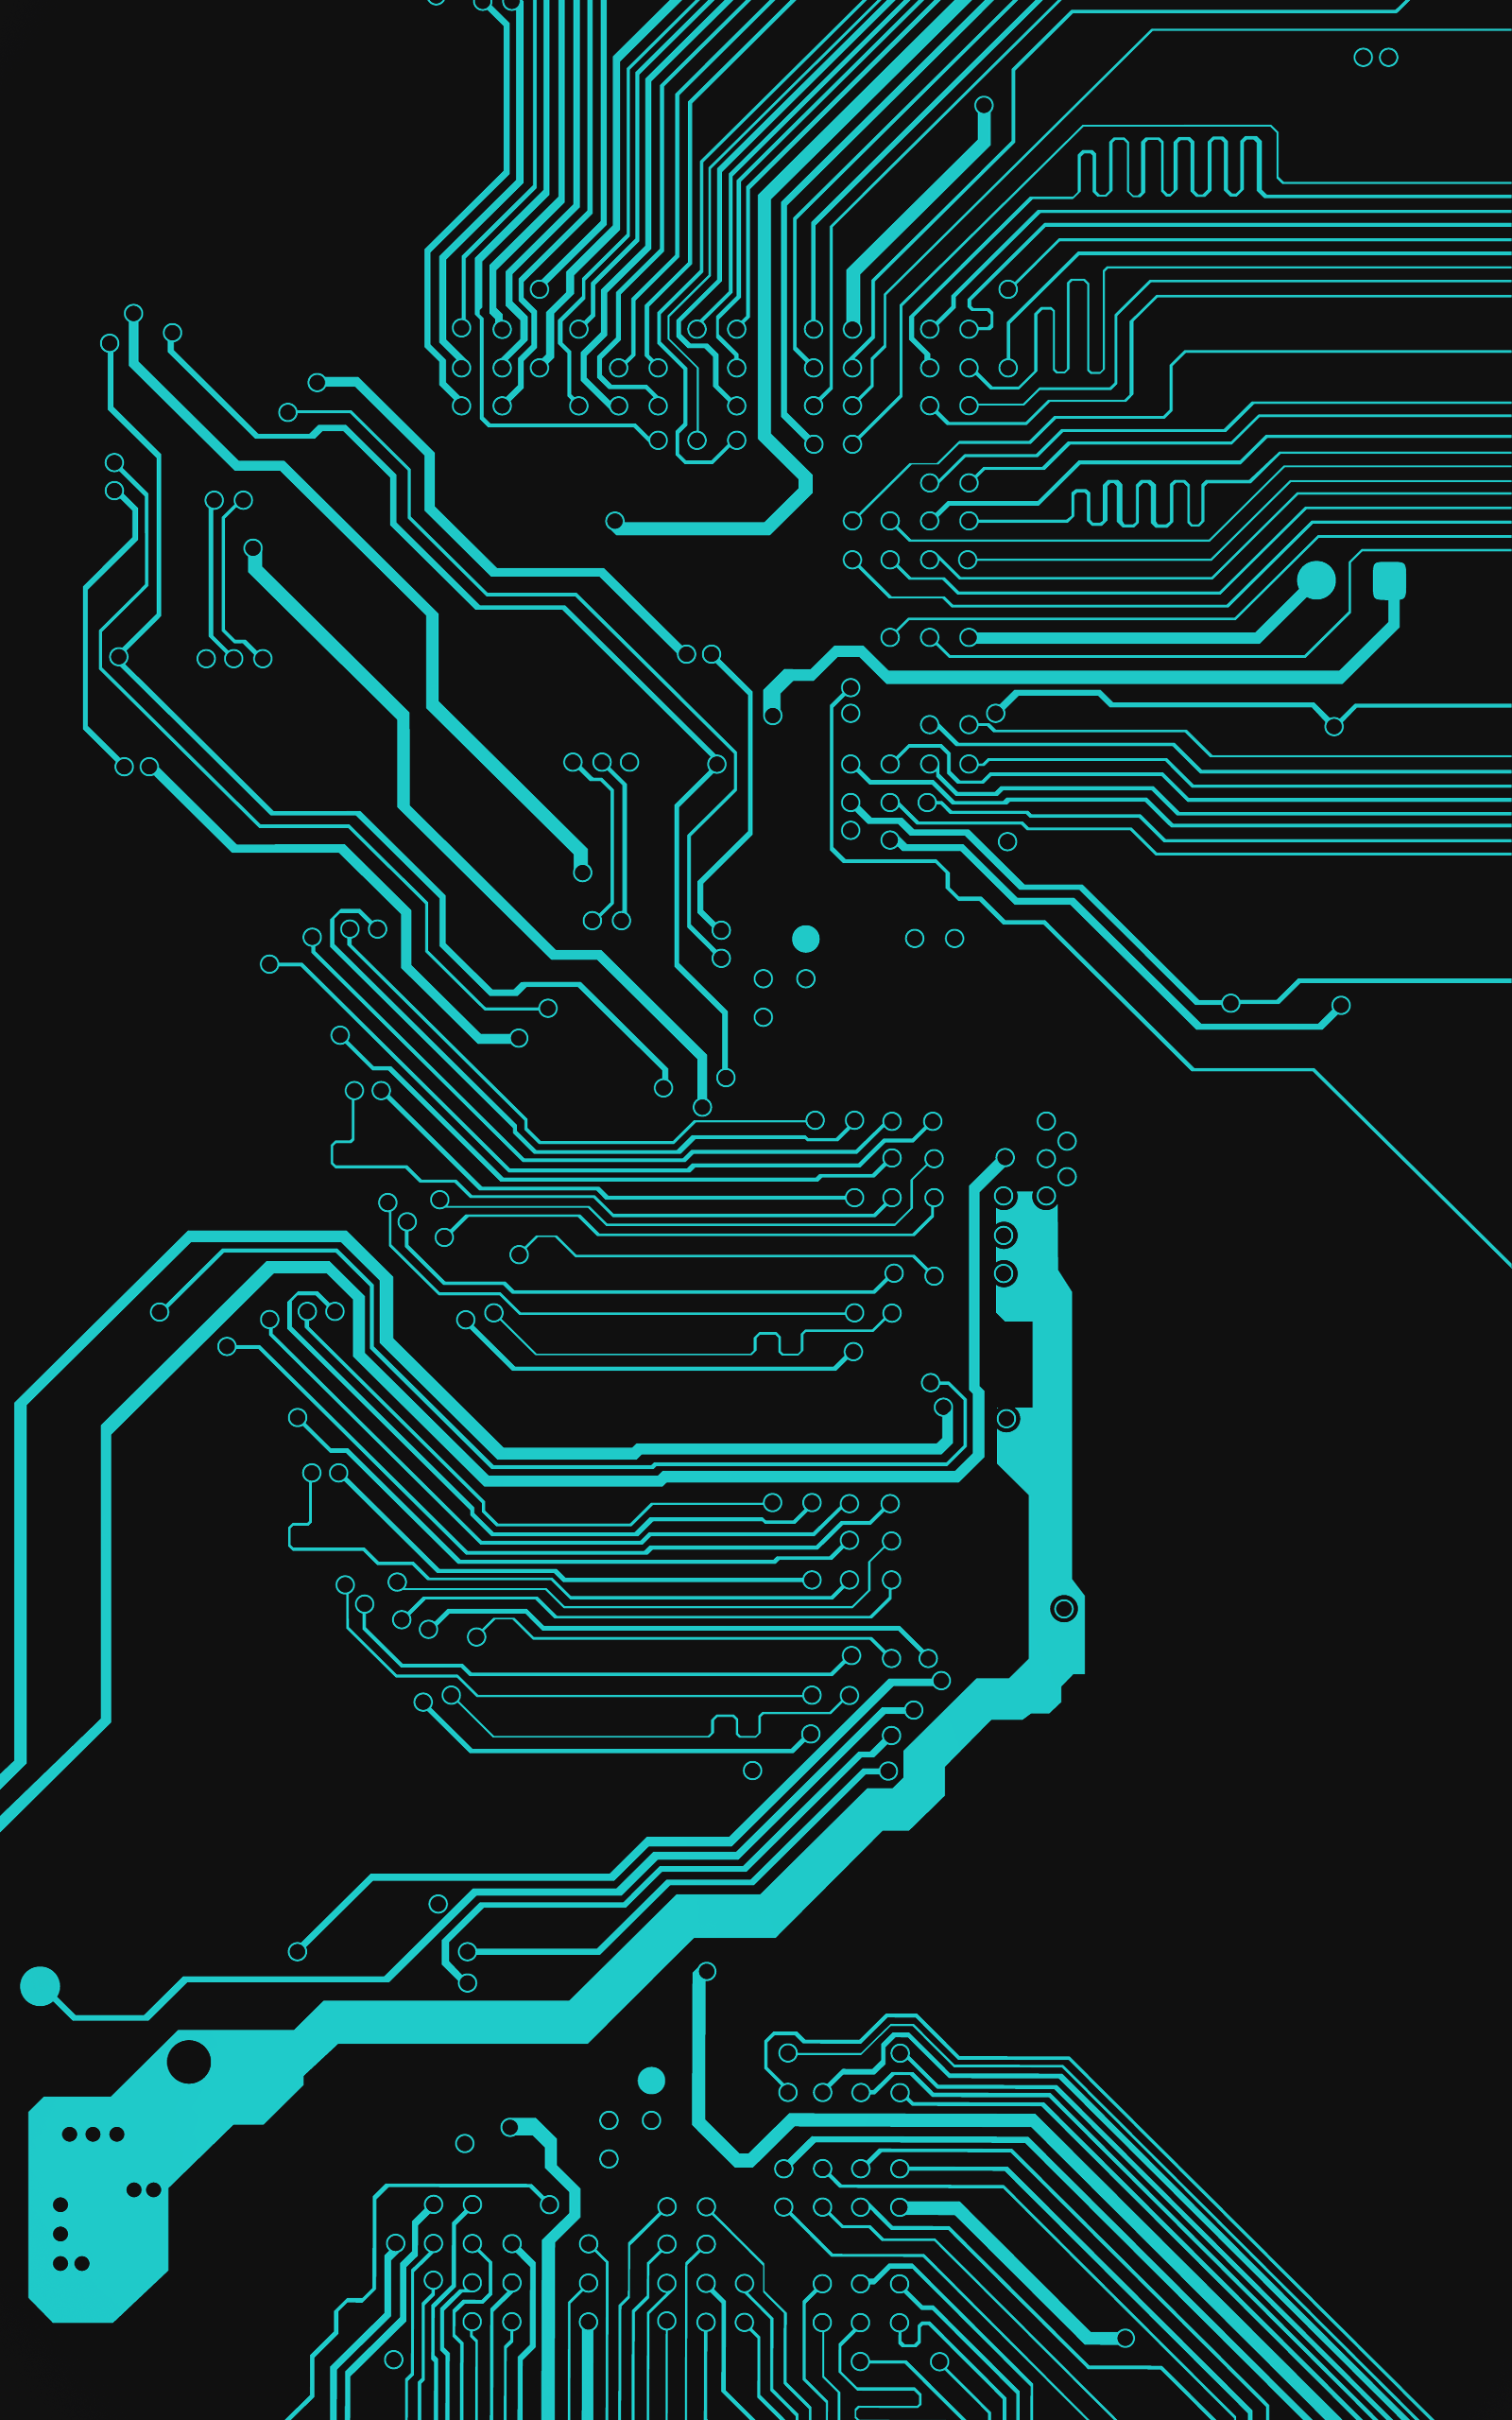
\includegraphics[width=\paperwidth]{background}}; % Background image
\draw[anchor=north] (midpoint) node [fill=ocre!30!white,fill opacity=0.6,text opacity=1,inner sep=1cm]{\Huge\centering\bfseries\sffamily\parbox[c][][t]{\paperwidth}{\centering How Processors Work ?\\[15pt] % Book title
{\Large A Very Gentle Introduction}\\[20pt] % Subtitle
{\huge Anurag Ghosh \& Parth Kolekar}}}; % Author name
\end{tikzpicture}};
\end{tikzpicture}
\vfill
\endgroup

%----------------------------------------------------------------------------------------
%	COPYRIGHT PAGE
%----------------------------------------------------------------------------------------

\newpage
~\vfill
\thispagestyle{empty}

\noindent Copyright \copyright\ 2016 Anurag Ghosh \& Parth Kolekar\\ % Copyright notice

%\noindent \textsc{Published by Publisher}\\ % Publisher

\noindent \textsc{https://github.com/stdarchsim/stdarchsim}\\ % URL

\noindent Licensed under the Creative Commons Attribution-NonCommercial 3.0 Unported License (the ``License''). You may not use this file except in compliance with the License. You may obtain a copy of the License at \url{http://creativecommons.org/licenses/by-nc/3.0}. Unless required by applicable law or agreed to in writing, software distributed under the License is distributed on an \textsc{``as is'' basis, without warranties or conditions of any kind}, either express or implied. See the License for the specific language governing permissions and limitations under the License.\\ % License information

%\noindent \textit{First printing, March 2013} % Printing/edition date

%----------------------------------------------------------------------------------------
%	TABLE OF CONTENTS
%----------------------------------------------------------------------------------------

%\usechapterimagefalse % If you don't want to include a chapter image, use this to toggle images off - it can be enabled later with \usechapterimagetrue

\chapterimage{chapter_head_1} % Table of contents heading image

\pagestyle{empty} % No headers

\tableofcontents % Print the table of contents itself

\cleardoublepage % Forces the first chapter to start on an odd page so it's on the right

\pagestyle{fancy} % Print headers again

%----------------------------------------------------------------------------------------
%	PRELIM
%----------------------------------------------------------------------------------------
%----------------------------------------------------------------------------------------
%	PART
%----------------------------------------------------------------------------------------

\part{Preliminaries}

%----------------------------------------------------------------------------------------
%	CHAPTER 1
%----------------------------------------------------------------------------------------

\chapterimage{chapter_head_2} % Chapter heading image

\chapter{Processors}

\section{Introduction}\index{Introduction}

Whenever we are playing any game like \textit{Crysis 3}, and the frame rate stutters, we exclaim, "\textit{This computer is so slow!}", without normally realizing the implications of what we say. What does it mean when we say a computing device is slow or fast ? How does a computing device actually perform computational tasks and instructions ?

Some of us may be aware that these computational tasks are performed by what is known as a Central Processing Unit or as are more commonly called, a Processor. 

\textbf{A processor carries out the instructions of a computer program by performing the basic arithmetic, logical, control and input/output (I/O) operations specified by the instructions.}

\begin{remark}
We would like to mention that not all computational tasks are performed by Processors, some tasks are delegated to other modules like Graphical Processing Units (GPU's), but we'll keep that out of scope of our discussion.
\end{remark}

The major aim of this book would be to understand how processors work and also learn the basic design principles that govern the design of a processor. 

We will be looking at processor design through a simple design and would study about various building blocks concerning that design. We would also learn some basic instructions that are a part of the processor design and also learn how these instructions are implemented and run in the processor.

For a hands on experience, we will also be writing some instructional level (called assembly) code for the processor design (on a simulator) and understanding how processors work at a very low level. As an aside, we'll also learn how our assembly code is translated to processor readable code and review different ways this is assembly is performed.

\newpage

%------------------------------------------------

\section{Brief History}\index{Brief History}

\begin{wrapfigure}{r}{0.4\textwidth}
\caption{EDVAC at Ballistics Research Lab}
\label{fig:edvac}
\centering
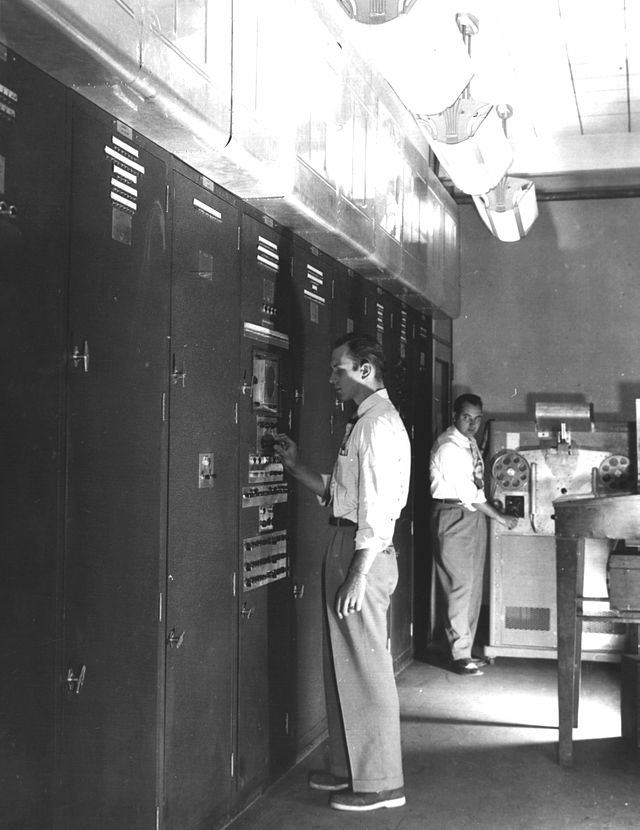
\includegraphics[width=0.4\textwidth]{EDVAC}
\end{wrapfigure}

Early computers like ENIAC were not programmable in nature in the sense of the word as we know it. To "program" these computers, one had to physically rewire them, which obviously was a very cumbersome process. Around the same time, the concept of "stored program" was floated around by John von Neumann through a report on EDVAC. 

EDVAC was designed to perform a certain basic instructions and programs written for EDVAC were to be stored in high-speed computer memory rather than specified by the physical wiring, which made writing programs and performing computational tasks much less cumbersome. These developments motivated the development of modern processors. 

Another architecture was popular in those times, known as the Harvard architecture. The key difference between the von Neumann and Harvard architectures is that the latter separates the storage and treatment of CPU instructions and data, while the former uses the same memory space for both. 

\begin{remark}
Most modern CPUs are primarily von Neumann in design, but CPUs with the Harvard architecture are seen mostly in embedded applications.
\end{remark}

With the advent of transistors, processor design grew increasingly more complex. Transistor-based computers had several distinct advantages over their predecessors. With increased reliability and lower power consumption, the CPUs operated at much higher speeds because of the short switching time of a transistor (from high to low and vice versa). 

\begin{wrapfigure}{l}{0.4\textwidth}
\caption{AL1, one of the first microprocessors}
\label{fig:edvac}
\centering
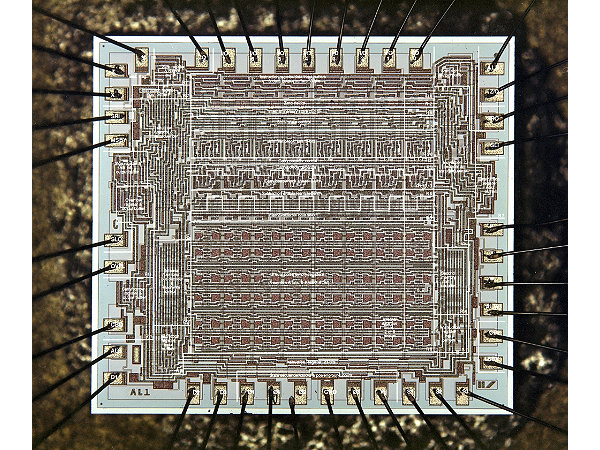
\includegraphics[width=0.4\textwidth]{al1}
\end{wrapfigure}

Transition was made from combining different components to building a System-on-Chip (SoC).  The integrated circuit (IC) allowed a large number of transistors to be manufactured on a "chip". Initially only basic circuits like NOR gates were miniaturized into ICs. CPUs based upon these IC's (building blocks) are generally referred to as small-scale integration (SSI) devices.

Further developments led to invention of techniques like Large Scale Integration, Very Large Scale Integration and finally, the Microprocessor. Previous generations of CPUs were implemented as discrete components and numerous small IC's on one or more circuit boards. Microprocessors, on the other hand, are CPUs manufactured on a very small number of IC's; usually just one.

\begin{remark}
Gordon E. Moore, the co-founder of Intel observed that the number of transistors in a dense integrated circuit doubles approximately every two years.
\end{remark}

While the complexity, size, construction, and general form of CPUs have changed enormously, the basic design and function hasn't changed much. Nearly all CPUs are von Neumann stored program machines.

%------------------------------------------------

\section{Basic Structure and Operation}\index{Basic Structure and Operation}



%----------------------------------------------------------------------------------------
%	PROCESSOR DESIGN
%----------------------------------------------------------------------------------------
%----------------------------------------------------------------------------------------
%	PART
%----------------------------------------------------------------------------------------

\part{Processor Design}

%----------------------------------------------------------------------------------------
%	CHAPTER 3
%----------------------------------------------------------------------------------------

\chapterimage{chapter_head_1} % Chapter heading image

\chapter{Presenting Information}

Machine oriented languages are more commonly known as assembly language. They are typically structured as one to one mappings to processor op codes (as we have seen earlier). However, assembly languages  also involve constructs (like psuedo instructions), macros and labels, all of which aid the programmers in writing programs and are not typically a one to one mapping to op codes.

\chapter{Microprogram Sequencer}

\section{Introduction}

We will start by defining a few terms

\begin{enumerate}
\item \textbf{Control Signal} It refers to the signal sent to a component (Register,ALU) to do a specific job. Also known as a Micro-operation. Example -
    \begin{enumerate}
    \item \textit{EPC} - Enable Program Counter To Bus,
    \item \textit{LOR} - Load Operand Register From Databus.
    \end{enumerate}
\item \textbf{Micro-instruction} The control signals are combined into control words, where each bit of the control word represents a signal. A control word is a micro-instruction. Example -
    \begin{enumerate}
    \item \textit{ EAR } \textit{LMR} ---- [MR] = [AR]
    \end{enumerate}
\item \textbf{Micro-program} A sequence of micro-instructions that are normally characterised by an assembly mnemonic i.e. an instruction.
\end{enumerate}

Now, A micro-program sequencer works in a way to generate these control signals from the microprogram by transitioning from one state to another in every clock cycle. A state is defined by the micro-instruction that has to be run in that clock cycle.It has two main functions 

\begin{enumerate}
    \item \textbf{Control Function} The micro-operations that need to be executed to perform a certain micro-instruction are to be defined and be known. The micro-operation(s) are dependent on parameters like selected destination, operand etc.
    \item \textbf{Sequencing Function} The address of next micro-instruction to be executed is generated while controlling test conditions etc.
\end{enumerate}

Thus, to summarize, to execute an instruction, the microprogram sequencer executes a micro-instruction in every clock cycle and determines which micro-instruction (state) to run next. It can be thought in terms of a state diagram.

\section{Work Flow}

\begin{figure}[h]
    \begin{center}
        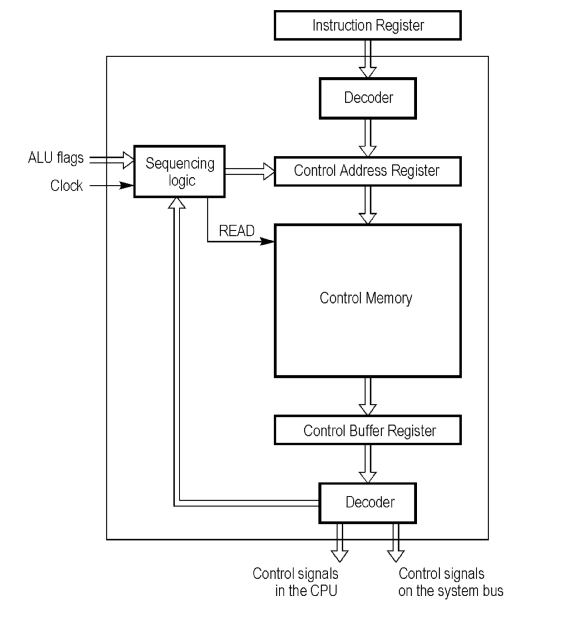
\includegraphics[scale=0.3]{MicroSequencer}
    \end{center}
    \caption{Flow of the Control Unit}
\end{figure}

The Instruction Register loads the opcode into the decoder which then translates the opcode into a control memory address. The control address register contains the address of the next micro-instruction to be read.

The micro-instructions are stored in the microprogram memory (also called control memory, can be used interchangeably). The address from the control address register is used to read from this microprogram memory.


When a micro-instruction is read from the microprogram memory, it is transferred to the control buffer register. This register activates the control signals.

\begin{figure}[h]
    \begin{center}
        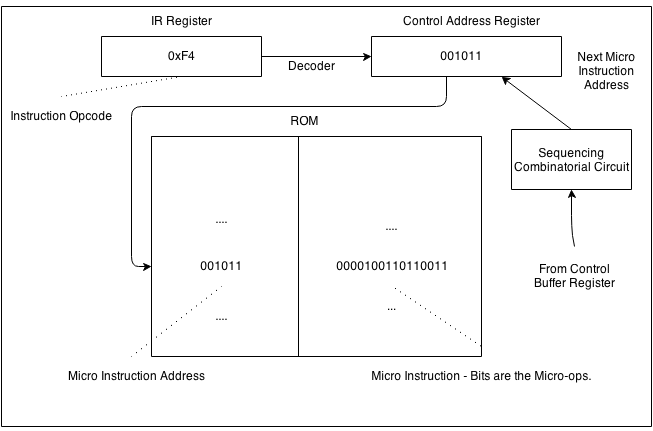
\includegraphics[scale=0.45]{SequencerTables}
    \end{center}
    \caption{The various addresses referred can get confusing.}
\end{figure}

\textit{I know you can see another decoder between the 
Control Buffer Register before the signals are sent. We will talk about this later.}
    
Thus, reading a micro-instruction from the microprogram 
memory has the effect of executing that micro-instruction.

The sequencing logic loads the control address register and 
activates the read signal. This read signal loads the next micro-instruction from the Instruction Register completing a cycle.

\section{Writable Control Memory}

Rather than storing the micro instructions in the ROM, if we would use Flash Memory or RAM, then the design has a Writable Control Memory. This has benefits including the ease of patching the microprogram and, for certain hardware generations, faster access than ROMs could provide. User-programmable Writable Control Memory allows the user to optimize the machine for specific purposes.

\section{Breadth in Microprogram Sequencer Designs}

\subsection{Horizontal and Vertical Programming}

We noticed that there was another decoder in Figure 1, this is the characteristic of a type of microcode architecture called Vertical Programming. The other variant Horizontal Programming, does not have the decoder circuit.

In horizontal microcode architecture, each control signal is represented by a bit in the micro instruction, while in the vertical microcode architecture, a set of true signals is represented in the micro instruction in a shorter form. Thus the decoder is used to convert this shorter code into true signals.

Practically, a diagonal architecture is used, combining both horizontal and vertical programming designs.

\subsection{Hardwired vs Micro-Programmed Control Units}

Hardwired control units are implemented through use of sequential logic units, using finite number of gates to generate specific results based on the last and the cuurent instruction, similar to what we have seen earlier in synchronous circuit design. Their design uses a fixed architecture—it requires changes in the wiring if the instruction set is modified or changed. Hardwired control units are generally faster than micro-programmed designs. However they are difficult to design as the instruction set starts to grow bigger. 

Microcode simplified the job by allowing the assembly instructions to be defined via microprograms rather than by circuitry. Even late in the design process, microprogram for an instruction could easily be changed, whereas hard-wired CPU designs were very cumbersome to change. Thus, this greatly facilitated CPU design.

\clearpage

\section{Example - Using IIIT Processor Instruction Set Architecture}

We will be taking an taking up an example code and stage by stage break it down into its components to understand the sequence.

Let us take the following
\begin{verbatim}    
movi r0
01
movs r0
\end{verbatim}
\textit{movi} corresponds to the 0x9* opcode family, thus \textit{movi r0} is 0x90 \\
\textit{movs} corresponds to the 0x7* opcode family, thus \textit{movs r0} is 0x70


These instructions can be broken down into, each of which will act as a state of the Microprogram Sequencer
\begin{enumerate}
\item 0x90 \textit{(movi r0)}
    \begin{enumerate}
    \item \textit{EPC, LMR, IPC}
    \item \textit{RD, LMS, LIO, LIR}
    \item \textit{EPC, LMR, IPC}
    \item \textit{RD, LRG, RMS; SRG = 0} 
    \end{enumerate}
\item 0x70 \textit{(movs r0)}
    \begin{enumerate}
    \item \textit{EPC, LMR, IPC}
    \item \textit{RD, LMS, LIO, LIR}
    \item \textit{ERG, LAR, RMS; SRG = PASSO}
    \end{enumerate}
\end{enumerate}

\textbf{\textit{The SRG is generated from opcode by the I/O register, and thus is not needed to be present in the Microprogram Memory.( We'll call it ROM after this)}}

The first two states are fetch in both the instructions and thus we assume here that they have been executed and now the next instruction, 1.(c) is going to be executed.

\begin{figure}[h]
    \begin{center}
        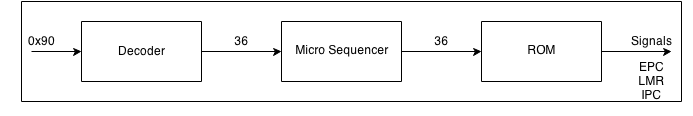
\includegraphics[scale=0.6]{InitFlow}
    \end{center}
    \caption{Flow of instruction 1.(c)}
\end{figure}

The states are stored in the ROM have a design dependent address. Let it contain state 2.(c) at address 34, 1.(c) at address 36 and state 1.(d) at address 37. The decoder has the said mapping of the states. The translated opcode ie, the address is fed to the Control Address Register which passes it to the ROM which then generates the signals. 

\begin{figure}[h]
    \begin{center}
        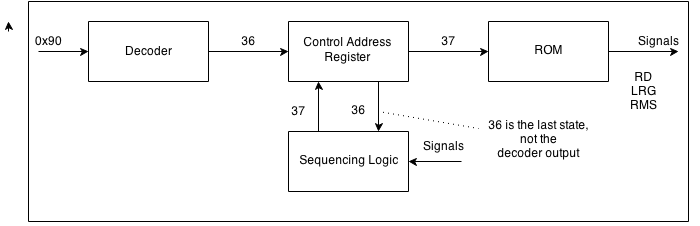
\includegraphics[scale=0.6]{SecondFlow}
    \end{center}
    \caption{Flow of instruction 1.(d)}
\end{figure}

\textbf{Also, the sequencing logic is then activated to change the address present in the Control Address Register to the next state.} The sequencer has thus jumped to the next state 1.(d).

The RMS control that is seen in this micro-instruction clear the Micro Sequencer to the reset value (ie. the initial state), usually zero.

\begin{figure}[h]
    \begin{center}
        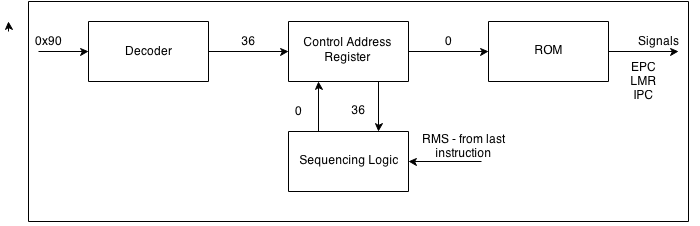
\includegraphics[scale=0.6]{FourthFlow}
    \end{center}
    \caption{Flow of instruction 2.(a)}
\end{figure}


\begin{figure}[h]
    \begin{center}
        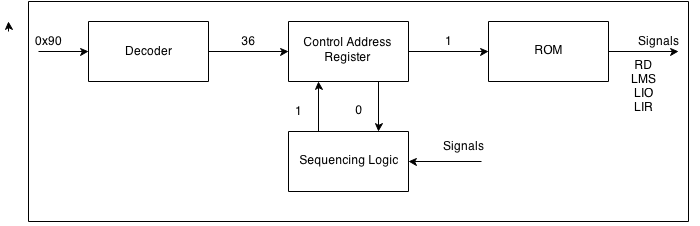
\includegraphics[scale=0.6]{FifthFlow}
    \end{center}
    \caption{Flow of instruction 2.(b)}
\end{figure}

\subsection{Coming Back to Fetch} \textbf{The states zero and one are maintained to be the fetch and decode micro-instruction cycles.} After RMS resets the sequencer state to zero, it again fetches the instruction in the next cycle by -

\begin{enumerate}
    \item At state zero, it will emit EPC LMR IPC to Load the Memory Address Register              with the value of the program counter.
    \item Then after state zero it will go to state one and emit RD LMS LIO LIR to load            the I/O Register, Instruction Register and the Micro Sequencer with the next
          instruction from the memory.
\end{enumerate}
Thus, the processor runs indefinitely till instructions are given.

\begin{figure}[h]
    \begin{center}
        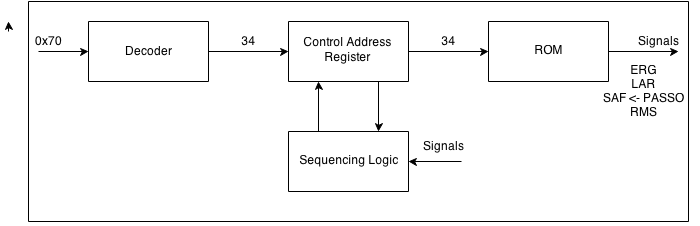
\includegraphics[scale=0.6]{ThirdFlow}
    \end{center}
    \caption{Flow of instruction 2.(c)}
\end{figure}

In the example the next instruction is \textit{movs r0}. Thus this instruction will cause the micro sequencer to change to the specific state with the micro-instruction. Thus the RMS of the prev instruction will cause state to be reset and the next instruction be fetched and executed.

\subsection{How and from Where the First Fetch ?} The initial state when the processor starts, is set to zero. Thus it fetches the instruction present at [[PC]] and executes it. Also, the PC is set to zero too and hence the first word from memory is fetched and executed on start up.

%----------------------------------------------------------------------------------------
%	ASSEMBLER
%----------------------------------------------------------------------------------------
%----------------------------------------------------------------------------------------
%	PART
%----------------------------------------------------------------------------------------

\part{An Introduction to Assemblers}

%----------------------------------------------------------------------------------------
%	CHAPTER
%----------------------------------------------------------------------------------------

\chapterimage{chapter_head_2} % Chapter heading image

\chapter{Assembler, Loaders and Compilers}

\textbf{An assembler translates a machine oriented language into machine language.} Machine oriented languages are more commonly known as assembly language. They are typically structured as one to one mappings to processor op codes (as we have seen earlier). However, assembly languages  also involve constructs (like psuedo instructions), macros and labels, all of which aid the programmers in writing programs and are not typically a one to one mapping to op codes.

\section{Compilers vs Assemblers}

In contrast to compilers, which are translators of languages which are machine independent in nature (have no direct mapping of instructions), assemblers are linked intrinsically to the architecture of the machine.

Architectural features such as memory word size, number formats, internal character codes, index registers, and general purpose registers, affect the way assembler instructions are written and the way the assembler handles instructions and directives. Such features are not taken in account by the compiler for higher level languages as they are built with architect agnostic features in mind.

\section{What are Loaders then ?}

Early systems had no concept of loading and linking executable and libraries. One only needed to assemble the program which would be directly loaded into the memory and run (as we saw previously in our processor simulator design). However, it was very easily seen that this cannot be a scalable model for execution. Many programs used certain sets of routines very frequently and it made no sense to write these routines every time one needed to write a program. A \textit{library} of such routines were developed along with methods to \textit{link} these routines to user code.
\textbf{Locating, loading, and linking of, assembling a single working program from individual pieces created the first assembler.}

Assemblers normally work in a two phase manner, they create a translated file from the input source known as \textbf{object file}. A loader then performs the loading, relocating, linking and starting the program from the object files (user object files, routine library files, etc).

\section{Relocation}

A program is assembled, the assembler does not know whether this is a complete program or part of a larger program. It assumes that the program will start at address zero and assembles it based on that assumption. Before the loader loads the program, it determines its true start address, based on the memory areas available at that moment and on the previously loaded object files. The loader then loads the program, making sure that all instructions fit properly in their memory locations. This process involves adjusting memory addresses in the program, and is called relocation.

\section{Benefits of Assembler Loader System}
Some of the benefits of such a system are as follows,

\begin{enumerate}
\item It makes it possible to write programs in separate parts that may also be in
different languages. Also, writing in separate parts leads in fewer bugs and higher readability.
\item When a change is made in the source code, only the modified program needs to
be reassembled. (Think of \textit{makefile})
\item The loader automatically loads routines from a standard library.
\end{enumerate}

\section{Bootstrapping}

One of the biggest questions that arises is, if you write an assembler in assembly language, how are you going to assemble it in the first place ?

This problem is solved by bootstrapping. What engineering do is that they write a very primitive assembler by hand, through manipulating op codes and then use that assembler to iteratively create a better assembler. Another method could be using a different system to write a software which cross assembles your assembler, but it's not very widely used.


%----------------------------------------------------------------------------------------
%	CHAPTER
%----------------------------------------------------------------------------------------

\chapter{Assembler Construction}

The input to any assembler is the source file. We would be talking about assemblers with respect to the assembly language that we have learned earlier. For our assembly language, each line consists of either certain instruction, a value for the previous instruction or a label.

\begin{lstlisting}[caption = Assembly Code Snippet]
movi r1
220
label: movs r1
load r2
\end{lstlisting}

In assembly languages used in industrial settings, normally there is a provision for comments and macros among other features (Assembly in such settings feels more like low-level C). We'll restrict our discussion to our bare-bones language for brevity. We will adopting a direct assemble-load model 
and wouldn't be discussing much about loaders.

\begin{figure}
\caption{A Typical Assembler}
\label{fig:assmblr}
\centering
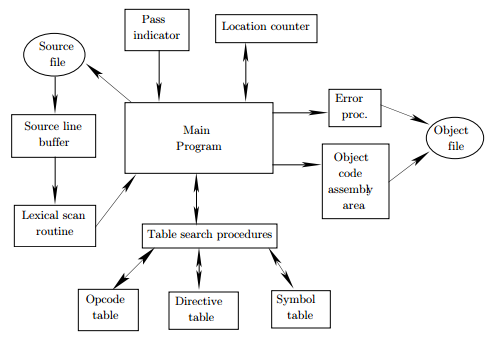
\includegraphics[width=0.4\textwidth]{assembler_block}
\end{figure}

\section{Deconstructing the Source File}

\subsection{Instructions}

The instructions normally are identified by the mnemonic and are directly mapped to some op code of the processor. The assembler is the one which defines this mapping through a table. It also keeps a track of structure of the intruction, ie. number of operands. 

Instructions can have zero, one, or two operands (some processors also have three operand instructions). The operands supply information to the assembler about the source line.
For example, \textit{movi} has 2 operands, the register in which we want to move and the value to be stored in it.

\subsection{Labels and References}

The label is necessary if we want to refer the instruction from some other point in the program. Now, where we refer to this label leads to two kind of references, "forward references" and "backward references". Forward References are those references where you refer to label that hasn't been defined yet (future label), if you read line by line from start. 

\begin{lstlisting}[caption = Forward Reference in Assembly]
jmpdnz
label
..
..
label: movs r1
load r2
\end{lstlisting}

Backward References are the ones that have been defined already. Obviously, future labels are not an error and their use should not be prohibited. The programmer should be able to refer to source lines which either precede or follow the current line. The problem of handling references is the core issue while writing Assemblers.

\section{Important Elements}

\subsection{OpCode Table}

To translate an instruction, the assembler uses the OpCode table, which is a static data structure. The two important columns in the table are the mnemonic and OpCode.

The OpCode table should be good for searching instructions. For each source line input, the assembler has to search the OpCode table. If it finds the mnemonic, it uses the OpCode to start assembling the instruction. It also uses the other information in the OpCode table, like number of operands etc to complete the assembly.

This table can be implemented in various ways, most notably using a hash table, which you will study in Data Structures if you haven't already.

\subsection{Symbol Table}

The symbol table is dynamic table that is used by the assembler, initially empty. Each entry in the table contains the definition of a label and stores the position of the label. Labels are added as they are encountered in the source file, and the table is also searched frequently to find the values of known labels, which is basically a reference to instruction number.

\newpage

\section{Two-Pass Assembler}

\begin{figure}[h]
\caption{A Typical Two Pass Assembler}
\label{fig:twopass}
\centering
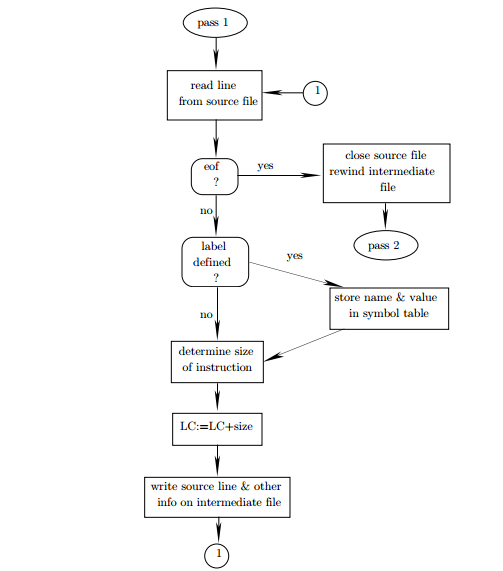
\includegraphics[width=0.6\textwidth]{two_pass_algo}
\end{figure}

A two-pass assembler is easier to understand and will be discussed first. Such
an assembler performs two passes over the source file. In the first pass it reads the
entire source file, looking only for label definitions. All labels are collected, assigned
values, and placed in the symbol table in this pass. No instructions are assembled
and, at the end of the pass, the symbol table should contain all the labels defined in
the program. In the second pass, the instructions are again read and are assembled,
using the symbol table. An assembler in our keeps
the size of each instruction in the OpCode table together with the mnemonic and
the OpCode



%----------------------------------------------------------------------------------------

\end{document}
